\documentclass[12pt]{article}
 
\newenvironment{sol}[1][Solution]{\begin{trivlist}\item[\hskip\labelsep {\bfseries #1:}]}{\end{trivlist}}
\usepackage{minted}
%\usemintedstyle{perldoc}
\usemintedstyle{vs}
\usepackage{graphicx}
\graphicspath{./}

\usepackage[margin=1in]{geometry} 
\usepackage{amsmath,amsthm,amssymb}
\usepackage{times,url}
\usepackage{tikz}
\usepackage{color}
\usepackage{enumerate}
\begin{document}
\renewcommand{\qedsymbol}{\filledbox}
\begin{center}
    \textbf{CS 5/7350 - Test\#2} \\
    \textbf{November 2, 2022}
%replace X with the appropriate number
\end{center}
\begin{flushright}
Name: \underline{Bingying Liang }\\
ID:  \underline{\ \ \ \ \ 48999397 \ \ \ \ \ }
\end{flushright}

\begin{enumerate}
    \item \ [9 pts] Consider heaps stored in an array:
    \begin{enumerate}
        \item How many swaps (maximum) may be required to insert an element into a heap stored as an array that currently has 3 integers?
        \begin{sol}
            2
        \end{sol}
        \item How many swaps (maximum) may be required to delete an element into a heap stored as an array that currently has 9 integers?
        \begin{sol}
        \begin{align*}
            \left \lfloor \log_2{9} \right \rfloor = 3
        \end{align*}
 
        \end{sol}
        \item How many swaps (maximum) may be required to create a heap from an array of 15 integers?
        \begin{sol}
            11
            \begin{center}
                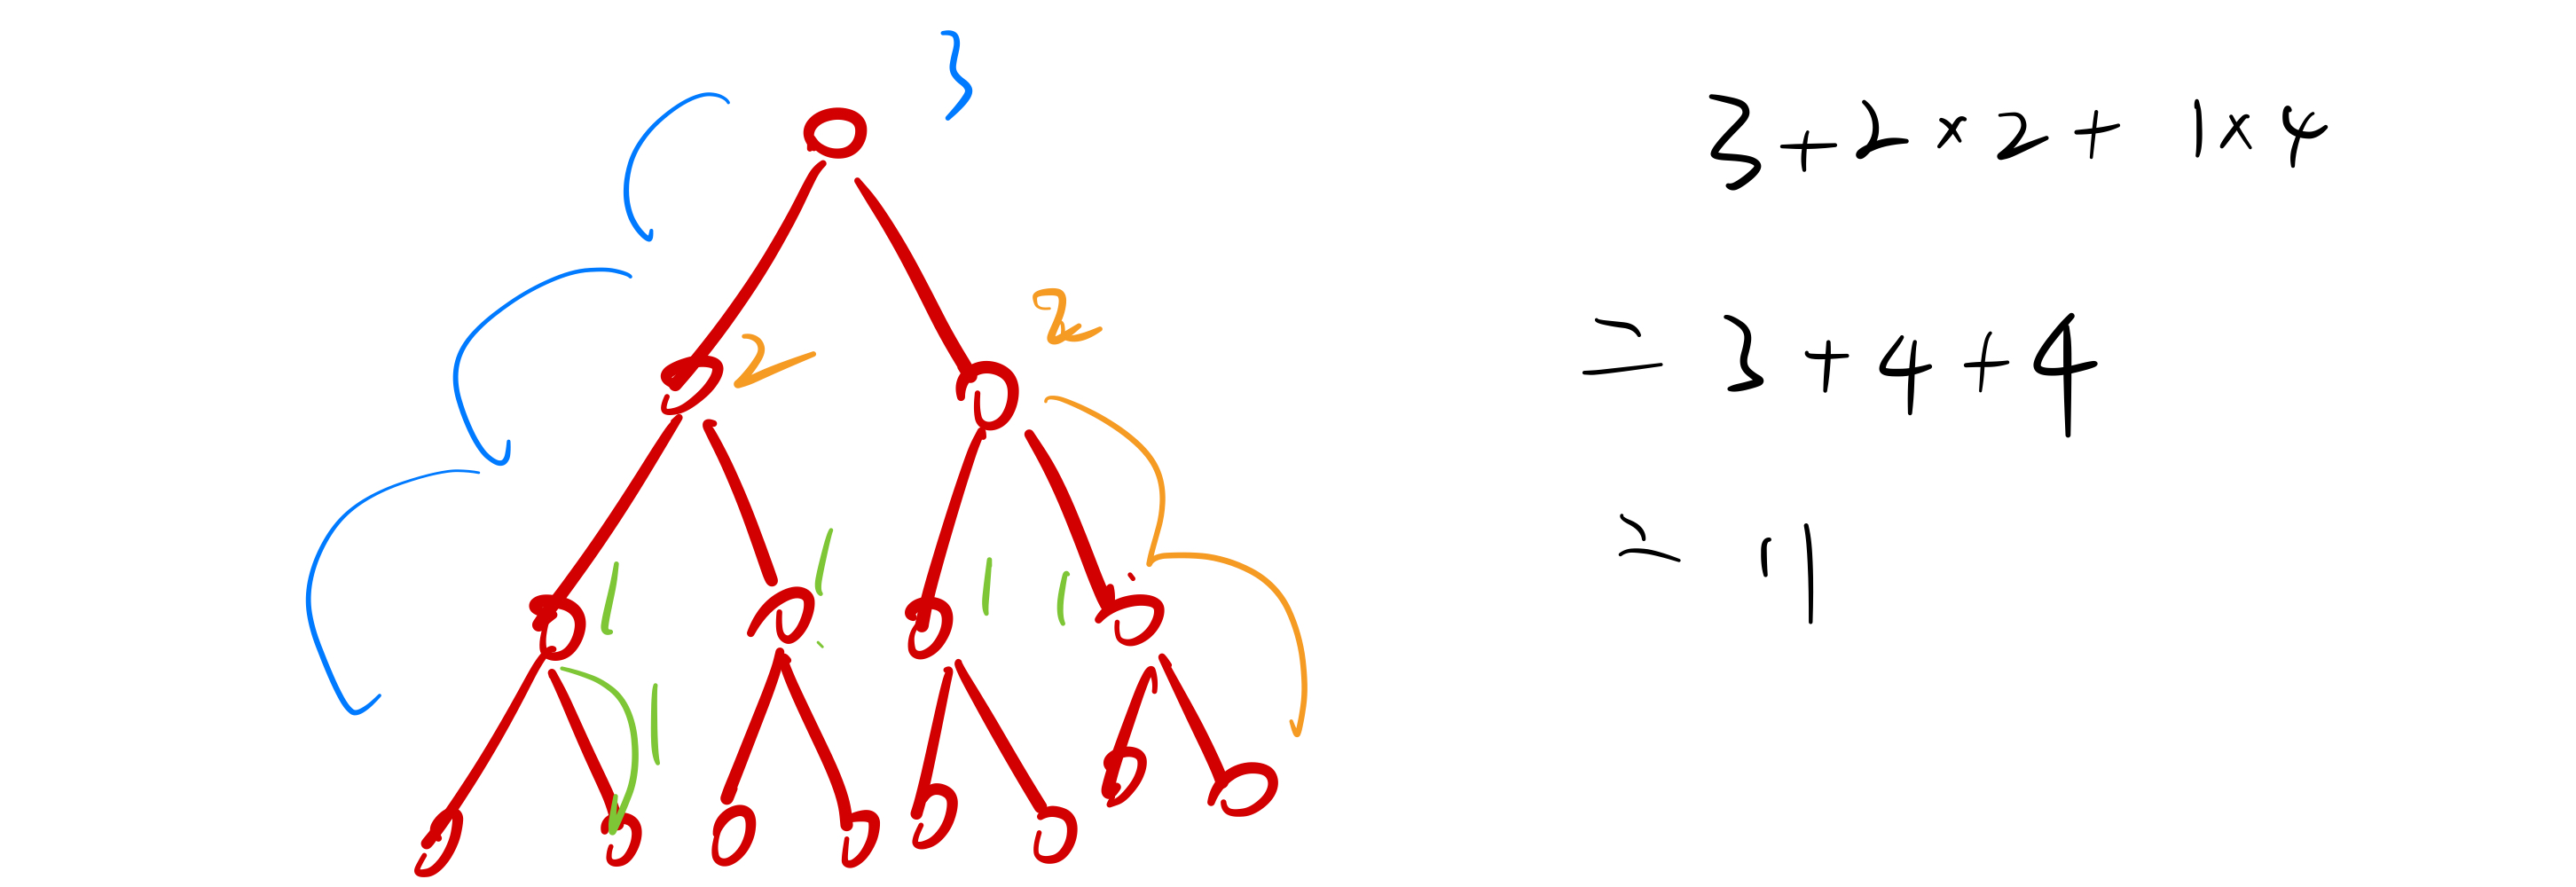
\includegraphics[width=0.9\textwidth]{p1.jpeg}
            \end{center}
        \end{sol}

    \end{enumerate}

    \item \ [6 pts] If a smallest last ordering has the largest degree when deleted of 13 and a terminal clique size of 11
    \begin{enumerate}
        \item What is the maximum number of colors that might be required by the ordering?
        \begin{sol}
        14
        \end{sol}
        \item What is the minimum number of colors that must be required by the graph?
        \begin{sol}
        11
        \end{sol}
    \end{enumerate}


    \item \ \textcolor{red}{[8 pts] When computing $n$ Choose $r(nCr)$, we can use the recursive equation of}
    \begin{align*}
        & _nC_r = _{(n-1)}C_{(r)} + _{(n-1)}C_{(r-1)}\\
        & \text{Note that } _nC_0 = 1 \text{ and } _nC_n = 1
    \end{align*}
    \begin{enumerate}
        \item Show pseudo code of how you would implement a nieve recursive function to compute $_nC_r$.
             \begin{sol}
        \hspace*{\fill}
        \begin{minted}[frame=lines,framesep=2mm,baselinestretch=1.2,fontsize=\footnotesize,linenos]{c}
choose(n,r){
    // base case
    if (r == 0){
        return 1;
    }
    
    if (n == 0){
        return 1;
    }
    // 
    return choose(n-1, r)+choose(n-1, r-1);
}
        \end{minted}
        \end{sol}
        \item What is the approximate asymptotic bound of the function representing the running time of your code?
        \begin{sol}
            \begin{align*}
                \Theta(2^n)
            \end{align*}
        \end{sol}
        \item Add a table to your recursive function to improve the running time.
        \begin{sol}
        \hspace*{\fill}
\begin{minted}[frame=lines,framesep=2mm,baselinestretch=1.2,fontsize=\footnotesize,linenos]{c}
T[n,r]  set T[0,r] = 1
        set T[n,0] = 1
choose(n,r){
    if T[n,r] = choose(n-1,r) + choose(n-1,r-1);
        return T[n,r]
    }
\end{minted}
        \end{sol}
        \item What is the new asymptotic bound of the function representing the running time of your code?
                \begin{sol}
            \begin{align*}
                \Theta(rn)
            \end{align*}
        \end{sol}
    \end{enumerate}
    \item \ [10 pts] Set up the table as shown in class for the Extended Euclidian Algorithm and compute 1/31 mod 12597

                  \begin{sol}
        \hspace*{\fill} \\
            \begin{center}
                \begin{tabular}{|c|c|c|c|c|c|c|}
                \hline
                     & A & B&Q &R &$\alpha$ & $\beta$  \\ 
                     \hline
                                       -1 &  & & & & 1 & 0 \\ 
                     \hline
                        & 12597 & 31 & 406 & 11 & 0 & 1 \\ 
                     \hline
                           &  31 & 11 & 2 & 9  & 1& -406 \\ 
                     \hline
                               &  11 & 9 & 1 & 2 & -2&  813  \\      
                     \hline
                             & 9 &2 &4 &1& 3& -1219 \\ 
                     \hline
                          & 2 &1 &2 &0 & -14& 5689 \\ 
                     \hline
                         & 1 &0 &- &-& 31 & 12597 \\ 
                     \hline

                \end{tabular}
            \end{center}
            \begin{align*}
                &(-14) \times(12599)  + 31 \times 5689 = 1\\
                &((-14) \times(12599)) \bmod 12599 +(31 \times 5689 )\bmod 12599 = 1\\
                & (31 \times 5689 ) \bmod 12599 = 1\\
                & \because (\frac{1}{31} \times 31) \bmod 12599  = 1 \\
                & \therefore \frac{1}{31}\bmod 12599  = 5689 \bmod 12599=5689 \\
            \end{align*}
        \end{sol}


    \item \ [5 pts] Show the swaps required to make a MIN heap using the HEAPIFY algorithm from the following array. Use one swap for each row in the table. Add extra rows if needed.
    \begin{sol}
    \hspace*{\fill}\\
            \begin{center}
        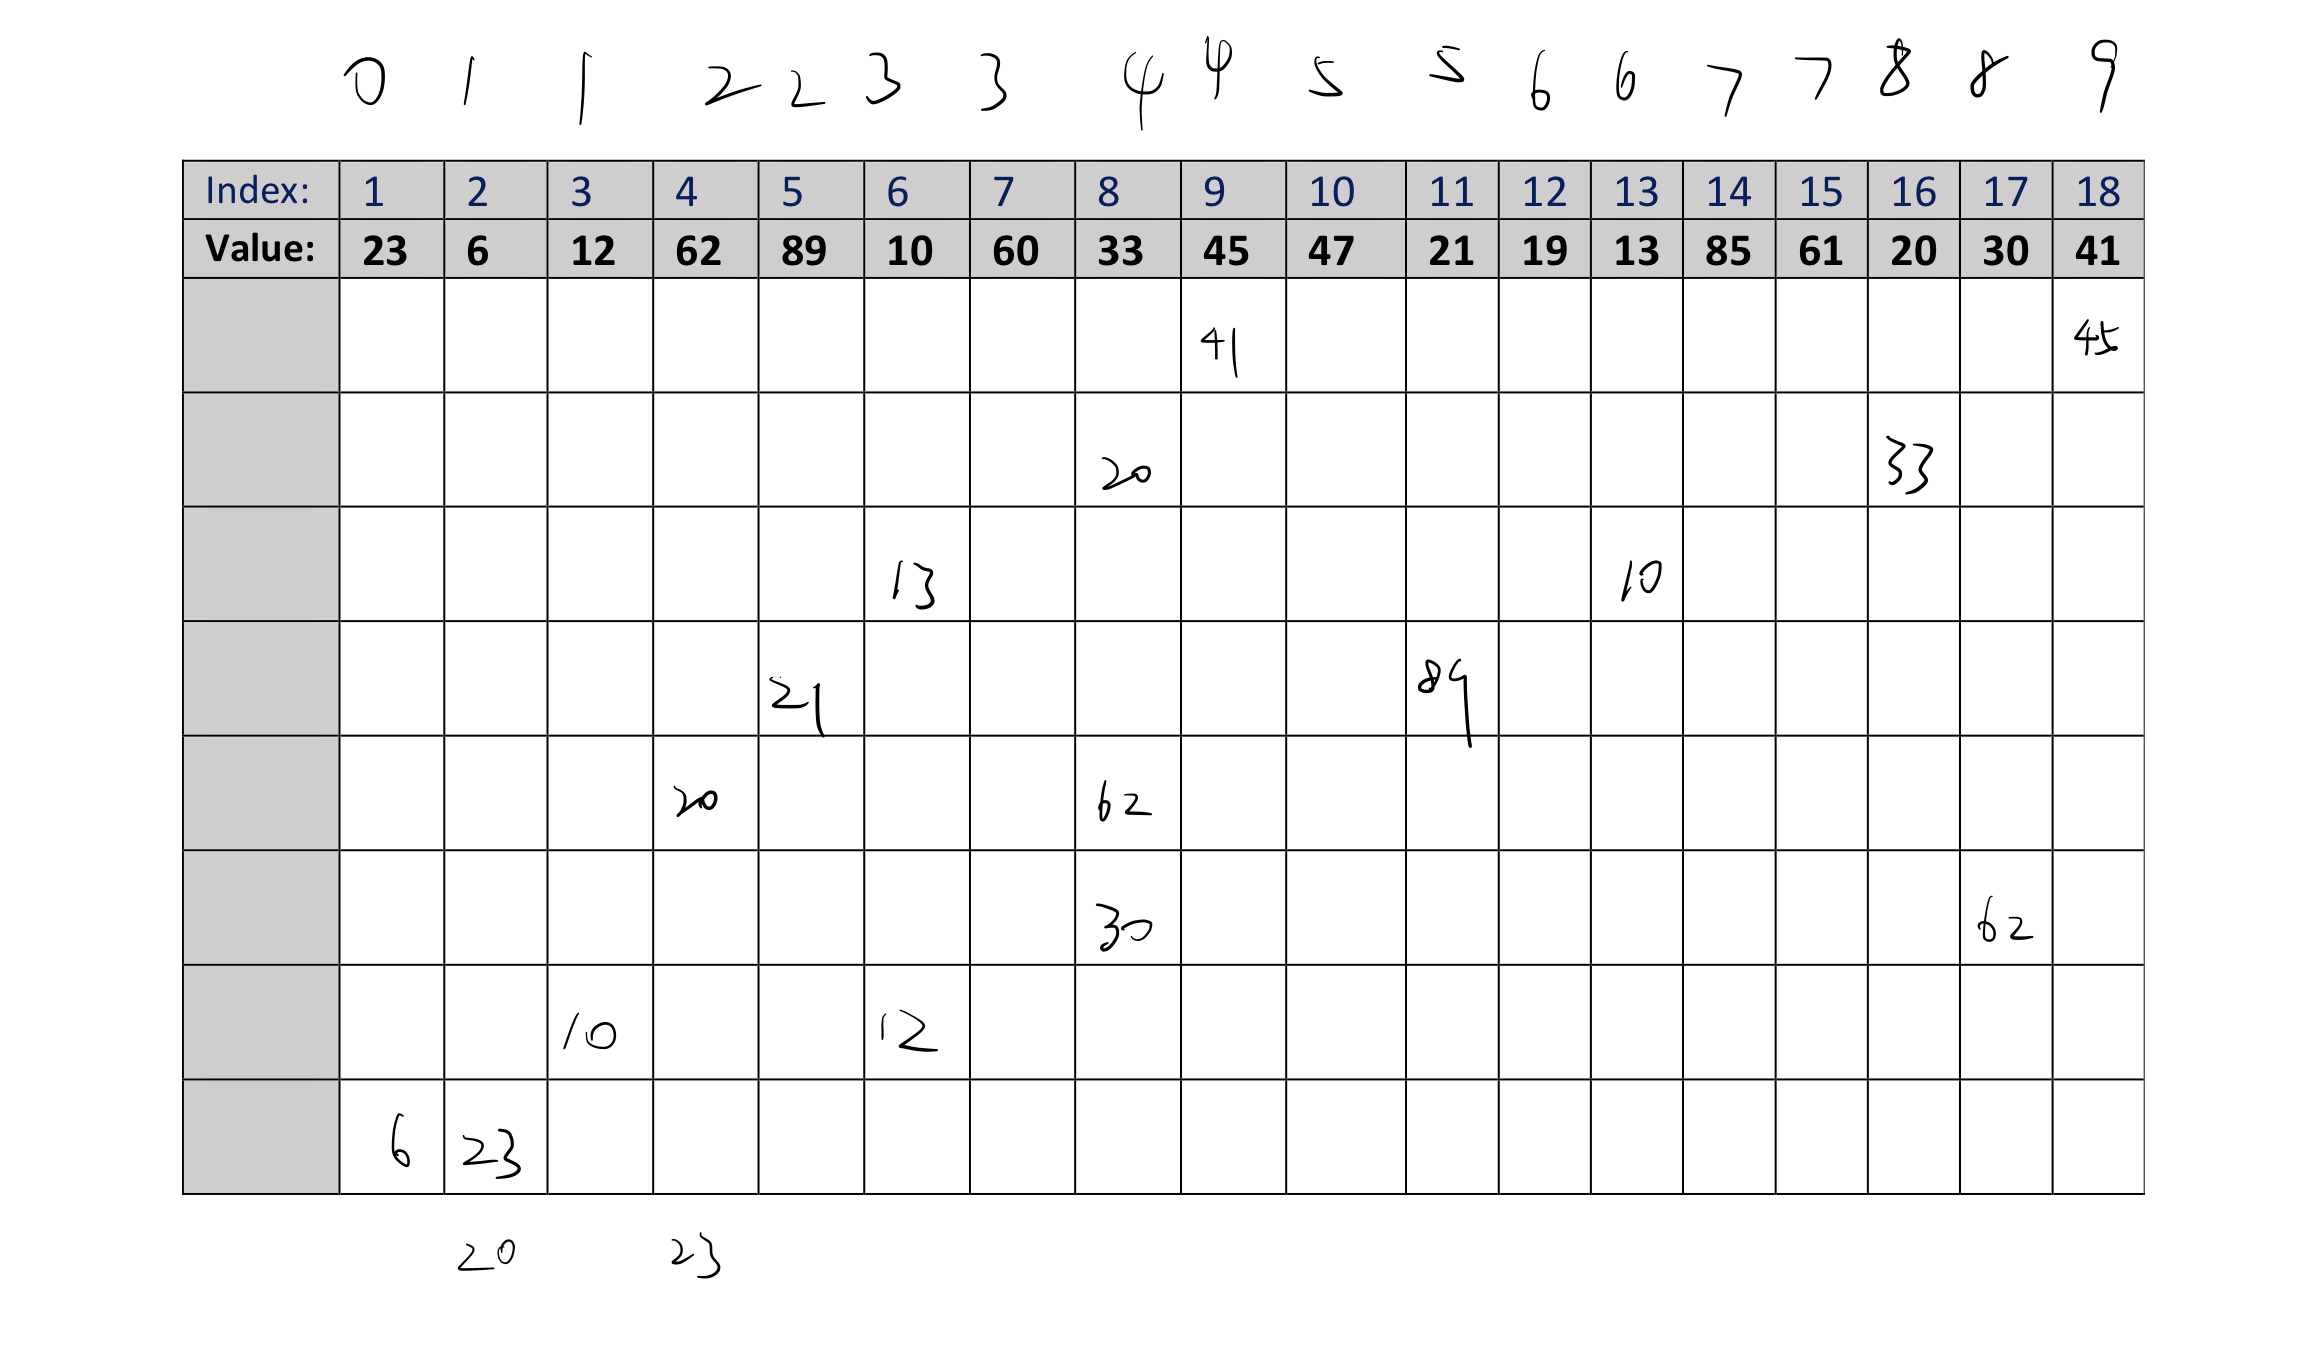
\includegraphics[width=0.9\textwidth]{p3.jpg}
    \end{center}
    \end{sol}

    \item \ [8 pts] Setup the table to find the longest increasing sub-sequence of the following sequence: 2 \ 5 \ 9 \ 6 \ 1 \ 7 \ 4 \ 8

    \begin{sol}
    \hspace*{\fill}
    \begin{center}
        \begin{tabular}{|c|c|c|c|c|c|c|c|c|c|c|}
        \hline
             2& 2& & & & & & & & & \\
                     \hline
             5& 2& 5 & & & & & & & & \\
                   \hline
             9& 2& 5 &9 & & & & & & & \\
                     \hline
             6& 2& 5& 6& & & & & & & \\
                     \hline
             1& 1& 5& 6& & & & & & & \\
                     \hline
             7& 1& 5& 6 &7 & & & & & & \\
                     \hline
             4& 4&5 &6 & 7& & & & & & \\
                     \hline
             8& 4& 5 & 6 &7 &8 & &  & & & \\
                     \hline
        \end{tabular}
    \end{center}
    The longest incraseing subsequence is 2, 5, 6, 7, 8 
    \end{sol}

    \item \ [6 pts] Draw a graph and give a smallest last vertex ordering of that graph where the terminal clique is not the largest complete subgraph. Circle the vertex you wrote down FIRST in the ordering.
    \begin{sol}
    \hspace*{\fill}
                    \begin{center}
        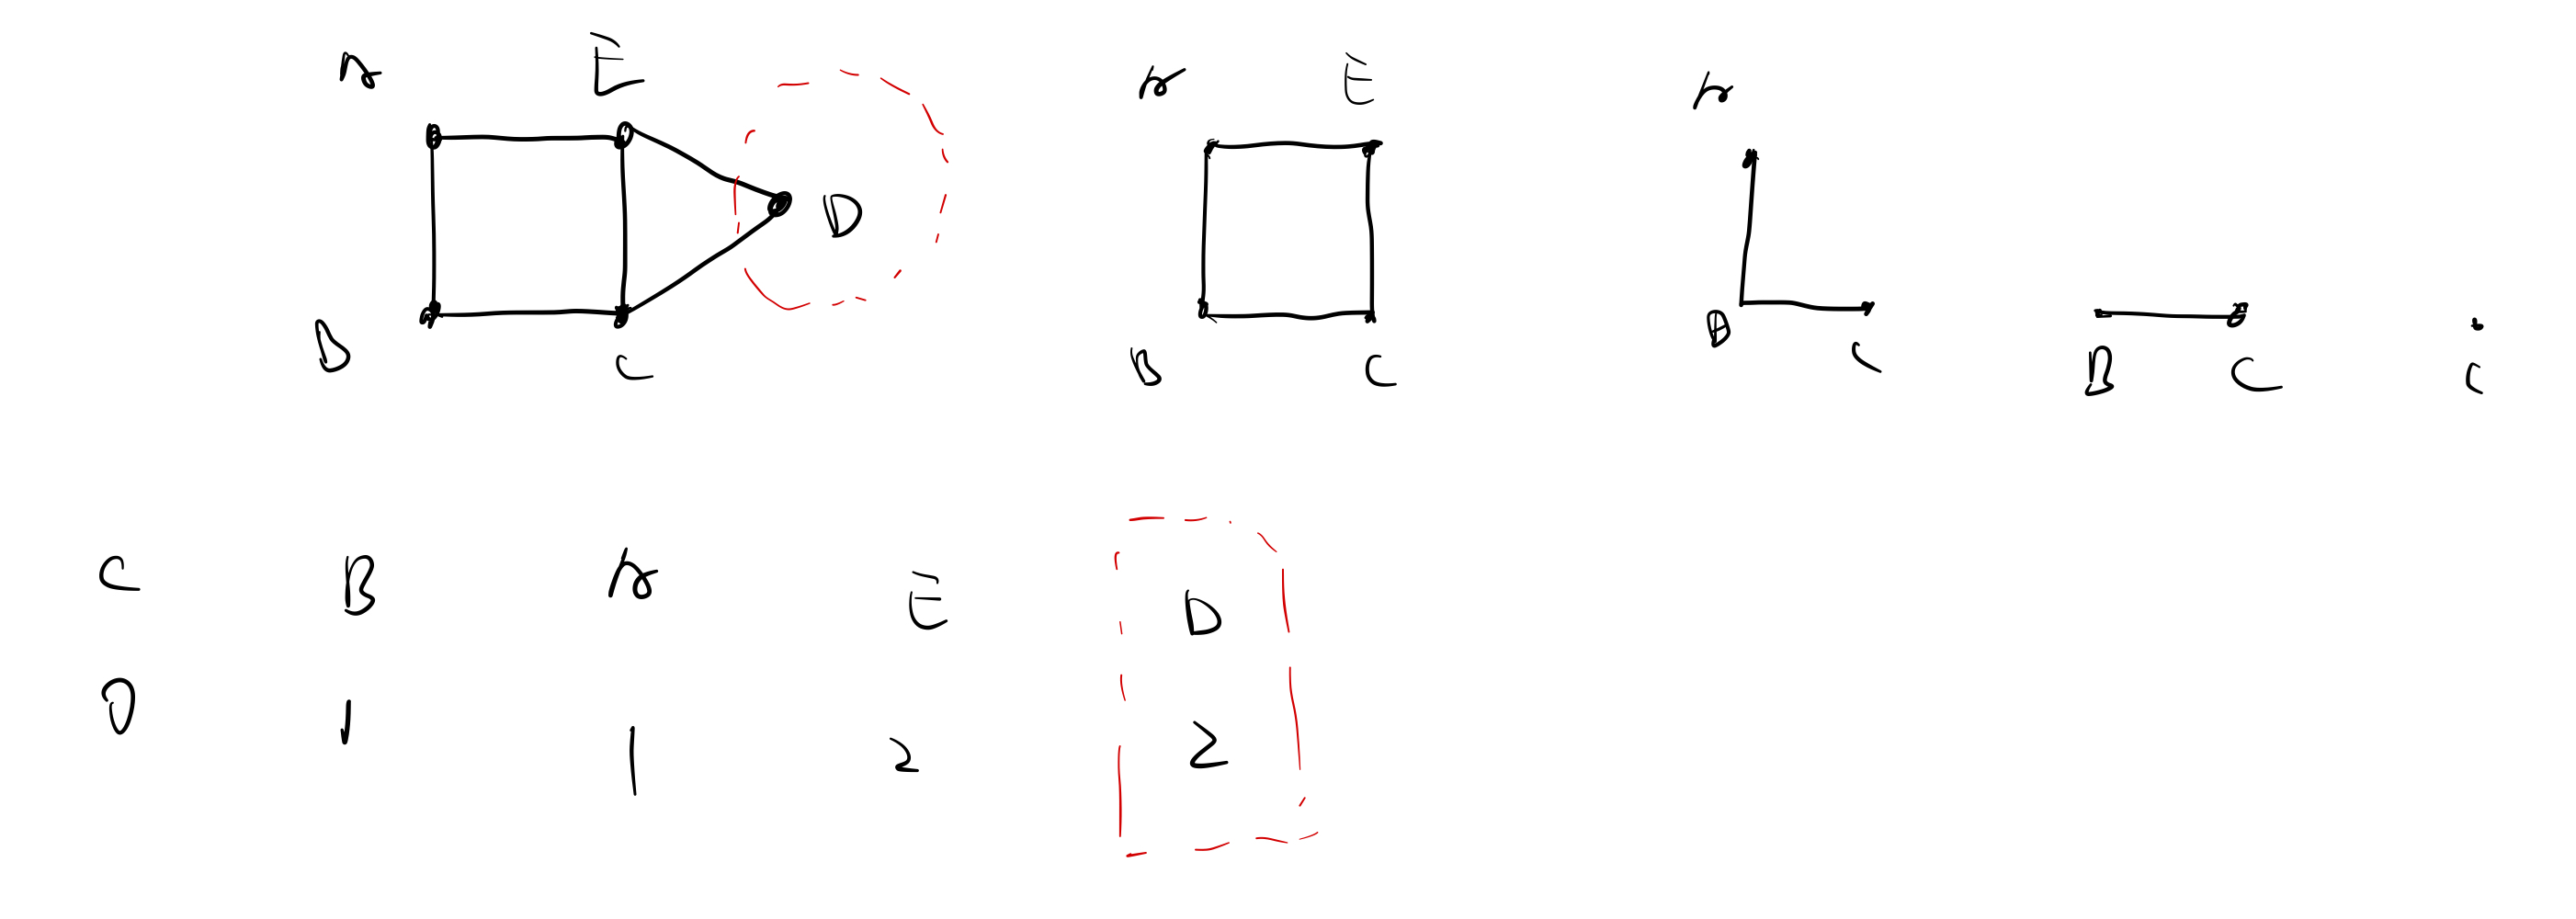
\includegraphics[width=0.9\textwidth]{p4.jpeg}
    \end{center}
    \end{sol}

    \item \ [8 pts] Set up a table to compute the length of the Longest Common Subsequence for the following two strings: 
    \begin{center}
        A  \ C \  T \ T \ C \ G \ C \ C \ and  \ C \ T \ A \ C \ G \ A \ C
    \end{center}

            \begin{sol}
        \hspace*{\fill}
        \begin{center}
            \begin{tabular}{|c|c|c|c|c|c|c|c|c|c|}
            \hline
                  &- & A  & C & T & T & C & G & C & C  \\
                  \hline
                 - &0 & 0  & 0 &0 & 0& 0 & 0& 0 & 0\\
                 \hline
                C & 0 & 0  & 1  & 1  & 1  &1 &1 &1 &1\\
                \hline
                T &  0 & 0  & 1  &2   & 2  & 2 & 2& 2&2\\
                \hline
                A &  0 &  1  & 1  & 2  & 2  &2 &2 &2 &2\\
                \hline
                C &  0 &  1& 2  & 2  & 2  &3 &3 &3 &3\\
                \hline
                G &  0 &  1 & 2  & 2  & 2  &3 &4 &4 &4\\
                \hline
                A &  0 &  1 & 2  & 2  & 2  &3 & 4& 4&4\\
                \hline
                C &  0 &  1 & 2  & 2  & 2  &3 & 4&5 &5\\
                \hline
            \end{tabular}
        \end{center}
        The Longest Common Subsequence: C T C G C
        \end{sol}
        

    \item \ [8 pts] Set up a table to compute the length of the Levenshtein Edit Distance for the following two strings:
        \begin{center}
        A  \ C \  T \ T \ C \ G \ C \ C \ and  \ C \ T \ A \ C \ G \ A \ C
    \end{center}
                \begin{sol}
        \hspace*{\fill}
        \begin{center}
            \begin{tabular}{|c|c|c|c|c|c|c|c|c|c|}
            \hline
                  &-  & A  & C & T & T & C & G & C & C  \\
                  \hline
                 - &0 & 1  & 2 & 3 & 4 & 5 & 6 & 7 & 8\\
                 \hline
                C & 1 & 2  & 1 & 2 & 3 & 4 & 5 & 6 & 7 \\
                \hline
                T &  2 & 2  & 2 & 1 & 2 & 3 & 4& 5&6\\
                \hline
                A &  3 & 2  & 3  & 2  & 2  &3 &4 &5 &6\\
                \hline
                C &  4 &  3& 2  & 3  & 3  &2 &3 &3 &5\\
                \hline
                G &  5 &  4 & 3  & 3  & 4  &3 &2 &3 &4\\
                \hline
                A &  6 &  5 & 4  & 4  & 4  &4 & 3& 3&4\\
                \hline
                C &  7 &  6 & 5  & 5  & 5  &4 & 4&4 &3\\
                \hline
            \end{tabular}
        \end{center}
        The Levenshtein Edit:
        1.remove A: CTTCGCC  \\
        2. replace T to A: CTACGCC \\ 
        3. replace C to A: CTACGAC
        \end{sol}

    \item \ [8 pts] You have received a message that was compressed with LZW. Remember that A=65, B=66, C=67, and D=68. The dynamic part of the dictionary starts with entry 256. The message you received was
    \begin{align*}
        66  \ 65 \ 66 \ 68 \ 257 \ 259 \ 260
    \end{align*}
    \begin{enumerate}
        \item What was the original message and what is your dictionary after decompression?
                \begin{sol}
        \hspace*{\fill}\\
        \begin{center}
        \begin{tabular}{|c|c|}
        \hline
             Dictionary  \\
             \hline 
             A = 65 \\
             \hline
             B = 66 \\
             \hline 
             C = 67 \\
             \hline 
             D = 68 \\
             \hline 
             ...\\
             \hline
             256 = BA \\
             \hline 
             257 = AB \\
             \hline 
             258 = BD \\
             \hline 
             259 = DA \\
             \hline
             260 = ABD \\
             \hline 
             261 = DAA \\
             \hline 
        \end{tabular}
        \\
        \begin{tabular}{|c|c|c|c|c|c|c|}
        \hline
            &start \ $w$ & read $k$ & entry & output & Dictionary add & next \ $w$  \\
            \hline
             0& - & 66 & B & B & &  B  \\
             \hline 
            1&  B & 65 & A & A & BA = 256 & A \\ 
            \hline 
            2&  A & 66 & B & B &AB = 257 & B \\
            \hline
             3&  B & 68 & D & D &BD = 258 & D \\ 
             \hline
            4& D & 257 & AB & AB &DA = 259 & AB \\
            \hline
             5& AB & 259 &DA & DA & ABD = 260 & DA \\ 
             \hline
            6& DA & 260 & ABD & ABD &  DAA = 261 & ABD \\
            \hline
             7&  &  &  & & & \\ 
             \hline

        \end{tabular}
                \end{center}
        The original message is: B, A, B, D, AB, DA, ABD
        \end{sol}
        \item Assuming 8 bits per character, how many bits were in the uncompressed message?
        \begin{sol}
            \begin{align*}
                11 \times 8 = 88 \ bits 
            \end{align*}
        \end{sol}
        \item Assuming the last entry of your dictionary was 2047, how many bits were in the compressed message
        \begin{sol}
            \begin{align*}
                &\log_2{(2047+1)} = \log_2{2048}=11\\
                & 7 \times 11 = 77 \ bits
            \end{align*}
        \end{sol}
        \item Why might a larger dictionary increase the size of the compressed file?
        \begin{sol}
            More bits per entry in the file.
        \end{sol}
    \end{enumerate}

    \item \ [8 pts]The Levensthein Edit Distance determines the edit distance between two strings when Addition, Deletion and Substitution are allowed all at a cost of 1.
Assume you have two strings: A and B. the $i^{th}$ character of A is Ai and the $j^{th}$ character of B is Bj.
    \begin{enumerate}
        \item When considering the $i^{th}$ character of A and the $j^{th}$ character of B, what is the formula you would use for determining the value placed in the table at location i,j?
               \begin{sol}
        \hspace*{\fill}
        \begin{minted}[frame=lines,framesep=2mm,baselinestretch=1.2,fontsize=\footnotesize,linenos]{c}
// base case
if (i == 0){
    T[i,j] = T[0, j];
}
if (j == 0){
    T[i,j] = T[i, 0];
}
if (Ai == Bj){
    T[i,j] = min{T[i-1,j]+1,T[i, j-1]+1, T[i-1,j-1]};
}else{
    T[i,j] = min{T[i-1,j]+1, T[i,j-1]+1,T[i-1,j-1]+1};
}
        \end{minted}
        \end{sol}
    \end{enumerate}
        You have been given a new, string processing system that requires 1 cycle to delete a character, 2 cycles to substitute a character and 1 cycle to add a character.
        \begin{enumerate}
            \item[(b)] When converting from string A to string B and considering the $i^{th}$  character of A and the $j^{th}$ character of B, what is the formula you would use for determining the value placed in the table at location i,j?
                   \begin{sol}
        \hspace*{\fill}
        \begin{minted}[frame=lines,framesep=2mm,baselinestretch=1.2,fontsize=\footnotesize,linenos]{c}
// base case
if (i == 0){
    T[i,j] = T[0, j];
}
if (j == 0){
    T[i,j] = T[i, 0];
}
if (Ai == Bj){
    T[i,j] = min{T[i-1,j]+1,T[i, j-1]+1, T[i-1,j-1]};
}else{
    T[i,j] = min{T[i-1,j]+1, T[i,j-1]+1,T[i-1,j-1]+2};
}
        \end{minted}
        \end{sol}
            \item[(c)] Fill in the table to determine the minimum number of cycles required to convert from string A = S G P Z T to string B = T S Z T M
                    \begin{sol}
        \hspace*{\fill}
        \begin{center}
            \begin{tabular}{|c|c|c|c|c|c|c|}
            \hline
                  &- & S & G & P & Z & T  \\
                  \hline
                 - &0 & 1& 2 & 3 & 4 & 5\\
                 \hline
                T & 1 & 2& 3 & 4 & 5 & 4 \\
                \hline
                S & 2 & 1&2 &3   & 4  & 5\\
                \hline
                Z &  3 &2&3 &4  & 3  & 4 \\
                \hline
                T &  4 &3 &5& 5 & 4  &3 \\
                \hline
                M &  5 &4 &5& 6  & 5  &4 \\
                \hline
            \end{tabular}
        \end{center}
        \end{sol}
            \item[(d)] Using your table above, what is the minimum number of cycles required to convert from string A = S G P Z T to string B = T S Z T M
            \begin{sol}
            4
            \end{sol}
        \end{enumerate}
    \item \ [8 pts] You have 3 different dice. Dice 1 has sides \{1,2,3\}. Dice 2 has sides \{2,2,2,3,3,3,4,4,4\} and Dice 3 has sides {2,3,3,4}. How many ways can you roll a 9 with these three dice? Set up the table for the dynamic programming algorithm and fill in the complete columns for Dice 1 and Dice 2. You may only fill in as much as you wish for Dice 3.
    \begin{sol}\hspace*{\fill}
        \begin{center}
            \begin{tabular}{|c|c|c|c|}
                \hline
                 sum / Dices & Dice 1 & Dice 1,2 & Dice 1,2,3 \\
                 \hline
                                1 & 1& 0& 0 \\ 
                 \hline
                                2&1 & 0&  0\\ 
                 \hline
                                3&1 & 3&  0\\ 
                 \hline
                                 4& 0& 6&  0\\ 
                 \hline
                                5& 0& 9&  3\\ 
                 \hline
                                 6 &0 & 6& 12 \\ 
                 \hline
                                  7& 0& 3&  24\\ 
                 \hline
                                  8& 0& 0& 30 \\ 
                 \hline
                                  9& 0& 0& 24 \\ 
                 \hline
            \end{tabular}
        \end{center}
    \end{sol}



    \item \ [8 pts] You have 2 different dice that are not evenly weighted:
    \begin{itemize}
        \item Dice 1 has sides {1,2,3} and a 10\% chance of rolling a 1, a 40\% chance of rolling a 2 and a 50% chance of rolling a 3.
        \item Dice 2 has sides {2,2,3,3,4,4} with a 15\% chance for each 2, a 15\% chance for each 3 and a 20\% chance for each 4
        \item What is the probability of rolling a 6 with these dice? Set up the table for
        \item the dynamic programming algorithm and fill in the complete column for Dice 1 and Dice 2.
    \end{itemize}
            \begin{sol}
        \hspace*{\fill}
        \begin{center}
            \begin{tabular}{|c|c|c|c|c|}
            \hline
                 & Die\#1 & Die \#2 & Die \#1,\#2\\
                \hline
                1& 10\% & 0  & 0 \\
                \hline
                2& 40\% &30\%  & 0\\
                \hline
                3& 50\% &30\% & 3\%\\
                \hline
                4 & 0 & 40\%  &15\% \\
                \hline
                5& 0 &0  & 31\% \\
                \hline
                6 & 0 & 0 & 31\%\\
                \hline
                7 & 0 & 0 & 20\%\\
                \hline
                Sum& 1 &1 & 1  \\
                \hline
            \end{tabular}
        \end{center}
        The probaility of rolling a 6 with these dice is 31\%.
        \end{sol}

\end{enumerate}

\end{document}
